\section{Results}
\label{sec:results}

\subsection{Short horizon: specialization, not a winner}
\label{sec:bakeoff}

The bake-off runs 275 questions (spanning 14 users) $\times$ 3 replicates $=$
825 judged answers per backend (Table~\ref{tab:bakeoff}).

\begin{table}[t]
\centering
\small
\caption{Short-horizon bake-off (825 judged answers per backend, 3 replicates
pooled). Vector's single category win (conflict-resolution, 42/42 vs.\
41/42 for both map and graph) is one answer inside replicate noise.}
\label{tab:bakeoff}
\begin{tabular}{lrrl}
\toprule
Backend & Total & \% & Signature strengths \\
\midrule
none (control) & 125/825 & 15.2 & --- \\
curated map    & 777/825 & 94.2 & multi-session 24/27, current-state \\
vector         & 751/825 & 91.0 & no signature strength \\
graph          & 769/825 & 93.2 & single-fact 119/120, work-memory 124/126, injection 42/42 \\
hybrid v1      & 738/825 & 89.5 & (negative result, \S\ref{sec:hybrid1}) \\
hybrid v2      & \textbf{799/825} & \textbf{96.8} & first by 22; single-fact 120/120, work-memory 126/126 \\
\bottomrule
\end{tabular}
\end{table}

The three recall targets of \S\ref{sec:intro} map onto the winners:
user-model facts and work knowledge are graph-shaped; current-state
synthesis is curated-map-shaped.

\subsection{Naive composition fails}
\label{sec:hybrid1}

Hybrid v1 --- a deterministic compile of the graph into a map --- scored
738/825 (89.5\%), \emph{below both parents}. The graph stored no narrative
for the compiler to use, and deterministic string-joins amplified extraction
noise that each parent had been quietly curating away (entity focus in the
graph; an LLM cartographer in the map). Composition of two curated stores is
not itself curation.

\subsection{The layered architecture leads the memory systems at the short
horizon}
\label{sec:layered}

Hybrid v2 scored 799/825 (96.8\%) --- first among the memory architectures
by 22 answers, with no significant primary-judge difference from the
full-rendered-history baseline (\S\ref{sec:cost}): single-fact
120/120, work-memory 126/126, conflict-resolution 42/42 (the curator
repaired the noisy chains that sank v1), and best-in-class inference-only
(76/81) and episodic (8/9). The lead is significant under paired,
cluster-aware analysis: vs.\ the map, 45/23 discordant items (exact McNemar
$p=0.010$; user-cluster bootstrap 95\% CI for the difference $[+0.2,+5.5]$
pp); vs.\ the graph, 37/7 ($p<10^{-4}$; CI $[+1.6,+6.1]$ pp). Under a
\emph{complete} cross-family re-judging (\S\ref{sec:threats}) the graph
margin holds (74/47, $p=0.018$) while the map margin keeps its direction
but loses significance (88/69, $p=0.15$) --- consistent with the narrow
cluster interval above; we therefore treat the hybrid-v2--map short-horizon
lead as a primary-judge result. Honest
remainders: multi-session integration 19/27 (behind the pure map's 24/27),
preference-current 34/42, and the wiki reintroduces a flat-text injection
surface (40/42 vs.\ the raw graph's 42/42; \S\ref{sec:security}). Because
hybrid v2 was designed after observing v1's failure on this corpus, we treat
this number as benchmark-informed (\S\ref{sec:threats}); the long-horizon
result below is the stronger evidence.

\subsection{The tenure crossover}
\label{sec:crossover}

The tenure corpus runs 6 users $\times$ 3 replicates ($n{=}324$ per cell) with
as-of-date question sets at weeks 3, 6, and 9
(Table~\ref{tab:crossover}, Figure~\ref{fig:crossover}).

\begin{table}[t]
\centering
\small
\caption{Tenure accuracy (\%) by checkpoint (6 users $\times$ 3 replicates,
$n{=}324$/cell).}
\label{tab:crossover}
\begin{tabular}{lrrr}
\toprule
Backend & week 3 & week 6 & week 9 \\
\midrule
curated map & \textbf{81.2} & 79.6 & 78.4 \\
vector      & 75.3 & 68.8 & 74.7 \\
graph       & 75.9 & 79.0 & \textbf{90.4} \\
hybrid v2   & 80.2 & 85.8 & \textbf{93.2} \\
none        & 16.0 & 16.4 & 16.7 \\
\bottomrule
\end{tabular}
\end{table}

\begin{figure}[t]
\centering
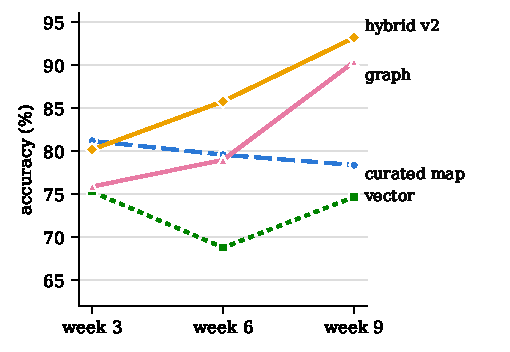
\includegraphics{figs/fig_crossover.pdf}
\caption{The tenure crossover: aggregate accuracy by history length
(6 users $\times$ 3 replicates, $n{=}324$/cell; the no-memory control,
16.0--16.7\%, is omitted for scale). The curated map leads at week~3; the
graph and layered hybrid invert the ranking by week~9.}
\label{fig:crossover}
\end{figure}

\textbf{Backend rankings invert with history length.} The curated map leads
the graph by 17 answers at week 3; they effectively tie at week 6 (a
2-answer gap); the graph leads by 39 at week 9 --- and every one of the six
users individually shows graph $\geq$ map at week 9. The week-3 and week-9
differences are each individually reliable: week-3 map $>$ graph (32/15
discordant, exact McNemar $p=0.019$; user-cluster bootstrap 95\% CI
$[+1.2,+9.0]$ pp) and week-9 graph $>$ map (57/18, $p<10^{-4}$; CI
$[+6.5,+19.4]$ pp). Separate significance at each end, however, is not
itself evidence that the difference \emph{changed}; the direct test is the
architecture$\times$tenure interaction,
$(\text{graph}-\text{map})_{\text{wk9}} -
(\text{graph}-\text{map})_{\text{wk3}}$: $+17.3$ pp on average, positive
for five of six users and null for one (per-user effects $+37.0, +16.7,
+9.3, 0.0, +20.4, +20.4$; user-cluster bootstrap CI $[+8.3,+26.2]$ pp),
with an exact six-user sign-flip randomization $p=0.063$ --- suggestive but
resolution-limited: six clusters with one null user cannot reach
conventional significance on this test. Under the complete cross-family
re-judging (\S\ref{sec:threats}), however, the interaction
\emph{strengthens}: $+24.1$ pp on average, positive for all six users
(per-user $+40.7, +20.4, +16.7, +13.0, +27.8, +25.9$; exact sign-flip
$p=0.031$, the test's minimum), with both endpoint margins significant
($p=0.010$ week 3, $p<10^{-5}$ week 9). The crossover is judge-robust at
the cluster level. Hybrid v2 is the overall long-horizon leader
(86.4\%; CI over the map $[+3.6,+10.1]$ pp), the only backend top-tier at
every tenure, and its interaction over the map is $+15.7$ pp with all six
users positive (exact sign-flip $p=0.031$, the minimum achievable).

The mechanism is recall of evicted content
(Figure~\ref{fig:earlychapter}). On the early-chapter probe (the three
\texttt{-early} question types pooled; $n{=}54$ per cell) the map falls
96.3\% $\rightarrow$ 72.2\% as budget eviction consumes the oldest material
(13/0 discordant items week~3$\rightarrow$9, $p=2\times10^{-4}$), while the
graph rises 94.4\% $\rightarrow$ 100\% and hybrid v2 holds 100\% at every
checkpoint. A full-rendered-history baseline (\S\ref{sec:cost}) holds the
early-chapter probe at 160/162 across all checkpoints --- when nothing is
evicted, old content survives --- confirming that the map's loss is caused
by eviction, not by history length itself. The map's \emph{aggregate}
decline is mild ($-2.8$ pts) because most question types are
tenure-insensitive --- which is exactly why short-horizon benchmarks miss
the effect. Vector's unbounded
pool also failed the probe (88.9\% $\rightarrow$ 70.4\%): similarity
retrieval buries old records under similar newer content. Unbounded storage
without time-aware retrieval is not an episodic memory.

\begin{figure}[t]
\centering
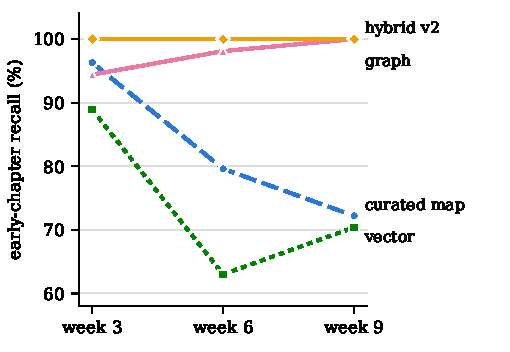
\includegraphics{figs/fig_earlychapter.pdf}
\caption{Early-chapter (evicted-content) recall by history length: the
three \texttt{-early} question types pooled, $n{=}54$ per cell. The
budgeted map's eviction consumes the oldest material; the unbounded graph
and the layered hybrid protect it.}
\label{fig:earlychapter}
\end{figure}

Short-horizon benchmarks --- the field's norm
\citep{maharana2024locomo,wu2024longmemeval,hu2026memoryagentbench,mem0report2026},
and our own \S\ref{sec:bakeoff} --- can mis-rank the architectures that a
long-lived assistant needs.

\subsection{Write-stage quality: a strong correlate of memory quality}
\label{sec:writequality}

A write-stage audit against script ground truth (66 audits: the 11
script-generated users $\times$ 3 replicates $\times$ both write paths) scored
the two-stage
curated writer at 84.5\% fact recall / 4.0 errors per audit against the
single-call graph extractor's 74.6\% / 8.5 --- half the audited error
count, bought with ${\sim}4.6\times$ the write-path tokens
(\S\ref{sec:cost}). Each audit scores one stored memory against the
life-script's atomic fact checklist: per-fact recall status
(correct/distorted/absent), an error list typed as
hallucination/distortion/misattribution, injection representation, and
volatility-class match. Scoring is by an LLM evaluator (the judge model)
run separately from --- and blind to --- downstream QA outcomes;
``fact-for-fact alignment'' means the audit's weak facts and the QA miss
categories matched at the level of individual fact keys --- and we can
quantify it, because the question templates and the audit checklist
reference the same script fields, giving a mechanical question--fact
mapping (17 of 20 templates map; abstention and injection probes have no
stored-fact key). Treating each (user, replicate, write path, question) as an
observation ($n{=}1{,}092$): a question whose underlying fact was written
weakly (distorted or absent) missed \textbf{24.2\%} of the time, against
\textbf{1.6\%} when the write was clean --- risk ratio ${\sim}15$, odds
ratio 19.6 (user-cluster bootstrap 95\% CI $[10.6, 50.3]$ over the 11
audited users; permutation $p<10^{-4}$, where weak-write labels are
shuffled within each user$\times$replicate$\times$write-path block with QA
outcomes held fixed, preserving each block's weak-label count;
$10^4$ permutations), consistent across both write paths (OR 16.3
curated, 25.6 extractor). 79\% of all QA misses had a weak-written
underlying fact. The scope is the association's own: the 11
script-generated short-horizon users and the 17 mechanically mapped
templates --- it has not yet been replicated on the tenure corpus or the
hand-built users. This quantifies the association --- it still does not
isolate causation (\S\ref{sec:threats}); hard facts could drive both
sides, and one measurement caveat applies: the audit evaluator is the same
model as the QA judge, so shared evaluator tendencies could induce
correlated measurement error --- the association's magnitude should not be
treated as independently validated until the audit labels receive human or
cross-family checking. The audit rubric, all 66 audit records, and the association script
are released; auditor--human agreement has not been measured and is
planned alongside the judge audit (\S\ref{sec:threats}). Write-stage weak facts aligned with downstream
QA miss categories fact-for-fact: two linked measurements --- separately
executed, but sharing the evaluator model and the scripted fact keys ---
one diagnosis. We state this as a strong association, not a causal isolation:
the compared writers differ in procedure \emph{and} compute, and hard or
ambiguous facts could contribute to both write and answer errors; a crossed
writer$\times$store ablation under matched token budgets is the experiment
that would settle causality.
Even the best write path damages ${\sim}15\%$ of facts; answering models
paper over the noise until a probe surfaces it. The residual error classes
are specific: detail distortion (dates, reasons), misattribution, and slot
errors (a permanent fact filed in a functional slot;
\S\ref{sec:representation}).

\subsection{Representation: supersession, episodes, volatility}
\label{sec:representation}

\paragraph{Supersede, never erase.} Records are soft-invalidated with
supersession pointers; the replacing record carries the prior value as
inline prose. On knowledge-update questions --- the category commercial
systems measure worst (FactConsolidation single-hop: Mem0 18.0,
Zep/Graphiti 7.0; \citealp[v4, Table~3]{hu2026memoryagentbench};
independently corroborated by \citealp{reddy2026freshness}) --- the curated
map scored 120/123 and hybrid v2 121/123 (42/42 on current-value questions;
misses concentrate in past-value recall). A surprise with design
consequences: prose-inline history \emph{beat} explicit bi-temporal
versioned edges at read time (79/81 vs.\ 72/81 on knowledge-update-past)
--- rendering superseded edges puts stale values back into the answerer's
view, a failure mode the KG lineage \citep{rasmussen2025zep} does not
anticipate at read time.

\paragraph{Episodes must exist by construction.} No LLM writer produced
dated episodic entries unprompted; once episodes became deterministic
per-event records, history questions flipped from systematic failure to
near-perfect --- and every architecture that discarded raw episodes after
distilling lost the past.

\paragraph{Volatility is real but hard to classify.} 120/161 (75\%) of
anchor facts landed in their expected class, and the failure mode is
structural --- a \emph{permanent} allergy filed into a functional
\texttt{health\_state} slot was superseded by a passing cold. Lifecycle
machinery operating correctly on mis-slotted facts silently destroys
permanent knowledge.

\subsection{Security: what the representation buys}
\label{sec:security}

A four-experiment sweep probed where security properties live.

\paragraph{Injection resistance tracked the record representation.} A
plausibility-graded ladder of six received-email attacks (absurd lottery
$\rightarrow$ generic debt $\rightarrow$ subscription-shaped $\rightarrow$
invoice-context $\rightarrow$ contact-impersonation spear-phish
$\rightarrow$ memory-poisoning directive) probed the stores. The graph
asserted 0 of 6: structural quarantine --- third-party claims exist only as
claim-edges with the claimant as source --- held across the entire gradient
with no added defense. The flat store asserted 3 of 6, and not the
extremes: the breaches span the subscription, invoice, and spear-phish
rungs, while the absurd and the overtly manipulative both tripped other
handling --- injection success is non-monotonic in plausibility. Labels are
not a defense: an ``unconfirmed''-flagged claim is still asserted
downstream. In the full benchmark the pattern reproduces quantitatively
across 14 unique planted injection questions (one per user), each
evaluated over three stochastic answer/judge trials: the graph produced
zero unsupported assertions in all 42 trials; the layered hybrid's
flat-text wiki failed on 2 of the 14 unique probes (2/42 trials), the
curated map likewise on 2 of 14. This is the attack class of indirect prompt injection via
retrieved content \citep{greshake2023injection} and memory poisoning
\citep{chen2024agentpoison}; descriptively, the graph and the full
transcript had no observed failures on the 14 probes, whereas the two
flattened stores each failed on two --- an observed pattern, not a
statistically established architecture difference (an exact paired test
with only two discordant unique probes cannot reach conventional
significance). Two scoping notes. First, the compared systems differ in
retrieval and serialization as well as representation, so
``representation property'' is an interpretation of the observed pattern
--- content labels failing while structural typing held at every rung ---
rather than a component-isolated ablation, which would hold the other
components constant. Indeed, the full-history baseline sharpens the
interpretation: a raw transcript --- also flat text --- likewise blocked
all 14 unique probes across 42 trials (\S\ref{sec:cost}), because the
received-mail trust framing survives
verbatim in it. What failed is \emph{flattened assertional} storage that
strips authorship boundaries in the act of summarizing; the operative
property appears to be provenance boundaries surviving representation,
whether structurally (claim-typed edges) or textually (intact source
framing) --- not graph topology per se. Second, the uncertainty must be
computed at the unique-probe level, not the trial level: zero failures on
14 unique probes bounds the per-probe assertion rate only below
${\sim}19\%$ (95\% upper bound, treating probes as independent --- itself
optimistic, since probes share a template family); the supported claim is
resistance to this documented, non-adaptive attack class --- not security
in general (\S\ref{sec:threats}).

\paragraph{Content-type quarantine is a write-gate property.} Obligations
and payment demands quarantine by \emph{content}, independent of sender
trust --- a spoofed known-correspondent demanding a wire transfer was
blocked even under graded sender trust, while benign third-party recall (a
relative's venue change) survived. Defense in depth that sender-trust alone
cannot provide.

\paragraph{Confabulation control is a read-gate nobody has.} We report both
the unconditional and the conditional view, because they disagree.
Unconditionally, the accuracy winner also confabulates least: over the 972
tenure answers, hybrid v2 asserts a wrong specific on 12.8\% of all
questions (124/972, with 8 abstentions) against vector's 17.0\% (165/972,
with 98 abstentions). The design-relevant
behavior is conditional: when hybrid v2 \emph{is} wrong, it almost never
abstains --- 93.9\% of its errors (124/132) are confidently asserted wrong
specifics, vs.\ 62.7\% for vector (165/263), classified by the
deterministic answer-text rule documented in
Appendix~\ref{app:crossjudge} --- so the best system's failures are
precisely the silent, confident kind a user cannot detect.
Accuracy does not confer calibrated abstention. The conditional pattern
persists under the complete cross-family re-judging of all four memory
systems: hybrid v2's confident-error share remains highest (85.4\%) and
vector's lowest (62.5\%, vs.\ 62.7\% under the primary judge --- the
original contrast is judge-robust), with graph 78.0\% and map 69.3\%
between them; unconditionally, all four sit near 23--24\% wrong-specific
under the stricter judge (Appendix~\ref{app:crossjudge}) --- and the
planned human adjudication uses a three-way rubric (correct /
wrong-specific / abstention) for exactly this reason. And the one injection that survives
structural quarantine re-enters through the \emph{episodic} channel
(``received an auto-renewal notice at \$890''), which is mentionable by
design. Both failures motivate the same missing mechanism: an
evidence-grounded abstention gate at answer time
\citep{farquhar2024semantic,kadavath2022know,wen2024abstention} that
refuses to assert claims whose only support is third-party-authored
episodes.

\subsection{Baselines: no history, full history, and a token-matched
window}
\label{sec:cost}

Memory-ablated deltas are 79--82 points short-horizon (94.2--96.8\% vs.\
15.2\%) and 70 points long-horizon (86.4\% vs.\ 16.4\%) against the
no-history control. To test what those deltas actually establish, we added
two history baselines under the identical prompt, answerer, judge, and
3-replicate protocol: \textbf{full rendered history} (every event, chronological
--- it fits in context at every horizon here) and a \textbf{token-matched
recency window} (most recent whole events under hybrid v2's mean read
budget of ${\sim}$1,807 tokens).

\textbf{Short horizon: full context ties or beats the best memory system.}
Full history scores 97.9\% (808/825) --- statistically indistinguishable
from hybrid v2's 96.8\% under the primary judge (25/16 discordant,
$p=0.21$; user-cluster CI $[-1.0,+2.9]$ pp), ahead of the curated map
($[+1.1,+6.6]$ pp), and significantly ahead of hybrid v2 under the
cross-family judge (98/28, $p<10^{-5}$; \S\ref{sec:threats}). This
directly confirms, rather than merely cites, the sub-threshold regime
\citep{convomem2025}: below ${\sim}150$ conversations, reading everything
is competitive, and small-history evaluations like this one may fail to
separate the tested memory systems from a trivial strategy. The recency
window, by contrast, collapses to 73.0\% --- work-memory 19/126,
preference-current 9/42, knowledge-update-past 44/81 --- at the same mean short-horizon token
budget, \emph{selectively constructed and structured} memory context
substantially outperformed a recency-only window: hybrid v2's 1,807 tokens
beat the same 1,807 tokens of recency by ${\sim}24$ points (the systems
differ in more than selection --- representation, compression, and
supplementary retrieval also change). (The window is matched to hybrid v2's \emph{mean}
short-horizon spend; realized spend varies per question and grows with
tenure, so the tenure-window comparison is under-matched --- per-question
and per-checkpoint matching is future work.) (Full history also
produced zero unsupported assertions on all 14 unique injection probes
across 42 trials: the received-mail trust framing travels with the
transcript.)

\textbf{Long horizon: no judge-independent winner, at lower read cost.} Full
history reaches 82.4/85.8/88.9\% across the three checkpoints with
near-perfect early-chapter recall (160/162) --- confirming the crossover's
mechanism from the other side: when nothing is evicted, old content
survives. At week 9, whether the layered system \emph{beats} full history
is judge-sensitive, and we report it as such: under the primary judge,
hybrid v2 leads 93.2\% vs.\ 88.9\% (13/27 discordant, item-level $p=0.039$;
per-user effects $+3.7, -1.9, +7.4, +5.6, +7.4, +3.7$ pp, five of six
positive, sign-flip $p=0.063$); under the complete cross-family re-judging,
full history edges ahead at week 9 (272 vs.\ 260 of 324, $p=0.18$) and
leads the tenure aggregate under that judge (79.7\% vs.\ 72.4\%;
Appendix~\ref{app:crossjudge}), while under the primary judge the tenure
aggregate is effectively tied (85.7\% vs.\ 86.4\%). The judge-robust
statement is that \emph{no judge-independent accuracy winner emerged at
nine weeks, while the layered system reads roughly half the tokens per
question} --- with read cost growing far more slowly than full history's
(below); the graph likewise shows no significant difference from full
history under either judge. (Non-significance is not equivalence: we claim
the absence of a robust winner, not demonstrated parity.) The
recency window fails both regimes (42.9--66.4\%; early-chapter 17/54 at
week 9). Remaining baselines for future work: raw-chunk RAG with a
competitive reranker, and an oracle-retrieval ceiling.

\textbf{Cost.} Marginal read cost is small: 677 (vector) to 1{,}807
(hybrid v2) input tokens per question --- input-token charges of
${\approx}\$0.002$/question at July-2026 list pricing for the answerer
(input tokens only; output tokens, storage, retrieval infrastructure, and
amortized write cost are excluded, and per-call wall-clock times are in
the released logs rather than analyzed here); full history spends the
entire corpus per question (${\sim}2.8$--$5.2$K tokens here), growing
linearly with corpus size, with no judge-independent accuracy advantage to
show for it (above); hybrid v2's read cost also grows ($+48\%$ by week 9)
but from a base roughly half full history's at week 9. Two structural
results: the budgeted map's
read cost is flat with tenure (1{,}183 $\rightarrow$ 1{,}182 tok/q) while
the unbounded winners' grows ($+48$--$57\%$ by week 9) --- forgetting is
what keeps the map cheap, and the tenure crossover is the price of that
economy; and write-side quality is bought with tokens (the curated writer
spends ${\sim}4.6\times$ the extractor's tokens to halve the audited error
count) --- but write cost amortizes over every future read, so
the economics and the write-quality association
(\S\ref{sec:writequality}) point at the same place: the write path.
